\documentclass[10pt,a4paper]{article}
\usepackage[latin1]{inputenc}
\usepackage[english]{babel}
\usepackage{amsmath}
\usepackage{amsfonts}
\usepackage{amssymb}
\usepackage{graphicx}
\usepackage{fancyhdr}
\usepackage{lastpage}
\usepackage{multirow}

%Include and define  c code
\usepackage{listings}
\usepackage{color}
\usepackage{textcomp}
\definecolor{listinggray}{gray}{0.9}
\definecolor{lbcolor}{rgb}{0.9,0.9,0.9}
\lstset{
	language=C,
	keywordstyle=\bfseries\ttfamily\color[rgb]{0,0,1},
	identifierstyle=\ttfamily,
	commentstyle=\color[rgb]{0.133,0.545,0.133},
	stringstyle=\ttfamily\color[rgb]{0.627,0.126,0.941},
	showstringspaces=false,
	basicstyle=\small,
	numberstyle=\footnotesize,
	numbers=left,
	stepnumber=1,
	numbersep=10pt,
	tabsize=2,
	breaklines=true,
	prebreak = \raisebox{0ex}[0ex][0ex]{\ensuremath{\hookleftarrow}},
	breakatwhitespace=false,
	aboveskip={1.5\baselineskip},
  columns=fixed,
  upquote=true,
  extendedchars=true,
 frame=single,
 backgroundcolor=\color{lbcolor},
}

\oddsidemargin  -0.5cm
\evensidemargin 0.0cm
\textwidth      17.25cm
\headheight     1.0cm
\headsep		0.7cm
\topmargin      -0.5cm
\textheight		22.0cm

\pagestyle{fancy}
\lhead{Exercise 5}
\chead{EEMB1}
\rhead{\thepage\ of \pageref{LastPage}}
\lfoot{Theis Christensen\\Paulo Fontes\\Dennis Madsen}
\cfoot{Team3}
\rfoot{\today}
\renewcommand{\headrulewidth}{0.4pt}
\renewcommand{\footrulewidth}{0.4pt}
\begin{document}
\part*{EMB 2010 Team3 Exercise3}
\section{Introduction}
This exercise is about controlling the backlight of the screen on the Embedded Artists board. 
The backlight should be controlled with an output pin from the LPC2478 setup as an PWM port.
The PWM driver should use PWM1[1] and connect it to pin 1.18 (this pin controls the intensity of the LCD displays backlight).
\subsection{Backlight circuit}

\begin{figure}[h!]		%Remember to put the h!, to not fuck the sections.
	\begin{centering}
 		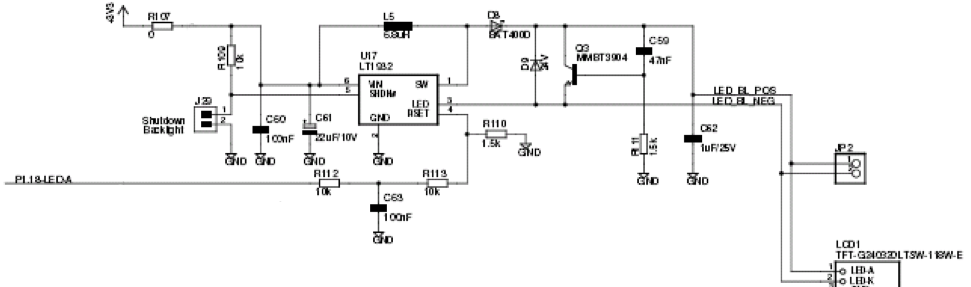
\includegraphics[width=1.0\textwidth]{backlight_circuit}
		\caption{The backlight device and the surrounding components to light up the backlight.}
	\end{centering}
\end{figure}

\subsection{Clock control}

\begin{figure}[h!]		%Remember to put the h!, to not fuck the sections.
	\begin{centering}
 		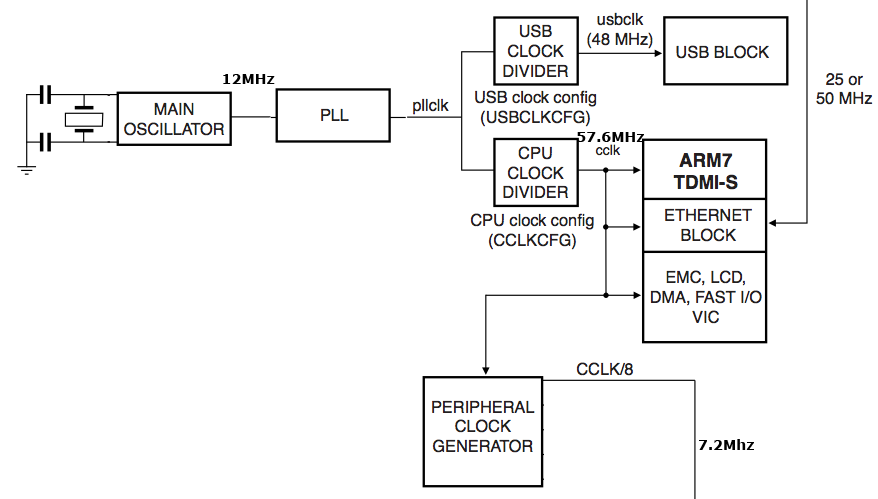
\includegraphics[width=0.8\textwidth]{peripheral_clock_gen}
		\caption{The routing of the clock inside the processor. Note that every unnecessary stuff is removed.}
	\end{centering}
\end{figure}
The input clock (crystal) runs at 12MHz. According to the config.h file found in the lpc2478-timer-irq project,
the Fcck (cclk on the diagram) is 57.6MHz when the USB is enabled (which it is). According to the data sheet of the
backlight a frequency of 5-40kHz should be provided. The clock is divided with 8 in the Peripheral clock (this is done in the 
initPwm function found in the pwm.c file). Now the PWM circuit is feed with a frequency of 7.2MHz. 
To get a frequency in the right range, the "period register" is set to 1000, which gives an output frequency of 7.2kHz. 
\section{Code}
\begin{figure}[h!]		%Remember to put the h!, to not fuck the sections.
	\begin{centering}
 		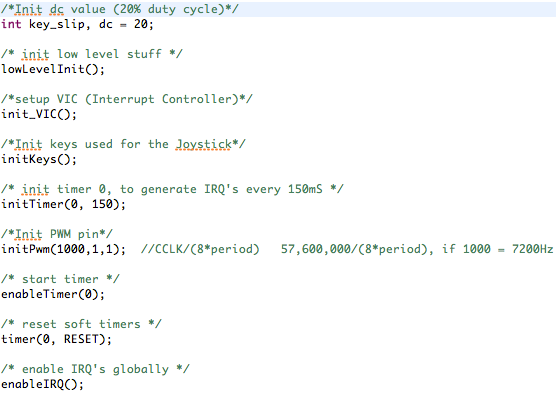
\includegraphics[width=0.7\textwidth]{main_init}
		\caption{Setup of the device; init functions is called in the start of main.}
	\end{centering}
\end{figure}

\newpage

\begin{figure}[h!]		%Remember to put the h!, to not fuck the sections.
	\begin{centering}
 		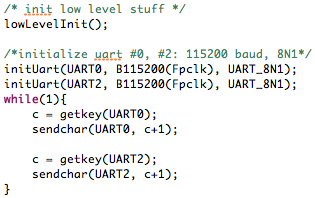
\includegraphics[width=0.35\textwidth]{main}
		\caption{The loop in the main function that the code continues executing.}
	\end{centering}
\end{figure}

Whenever the timer gives an interrupt (in this case every 150mS), the keys are read. Unfortunately the keys could not be setup with interrupts as the inputs used for the joystick does not support interrupt control.

\begin{figure}[h!]		%Remember to put the h!, to not fuck the sections.
	\begin{centering}
 		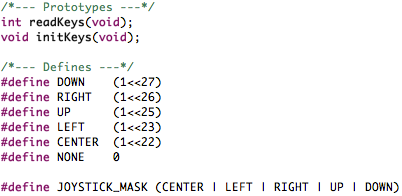
\includegraphics[width=0.5\textwidth]{keys_h}
		\caption{Defines of the joystick keys in the header file.}
	\end{centering}
\end{figure}

\begin{figure}[h!]		%Remember to put the h!, to not fuck the sections.
	\begin{centering}
 		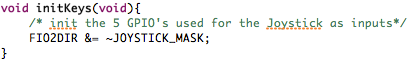
\includegraphics[width=0.55\textwidth]{init_keys}
		\caption{The 5 input keys from the joystick is set up as inputs.}
	\end{centering}
\end{figure}

\begin{figure}[h!]		%Remember to put the h!, to not fuck the sections.
	\begin{centering}
 		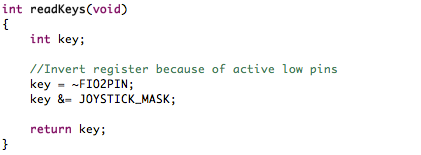
\includegraphics[width=0.6\textwidth]{read_keys}
		\caption{The function returns a value symboling the key pushed on the joystick. Zero is returned if no key is activated.}
	\end{centering}
\end{figure}

\begin{figure}[h!]		%Remember to put the h!, to not fuck the sections.
	\begin{centering}
 		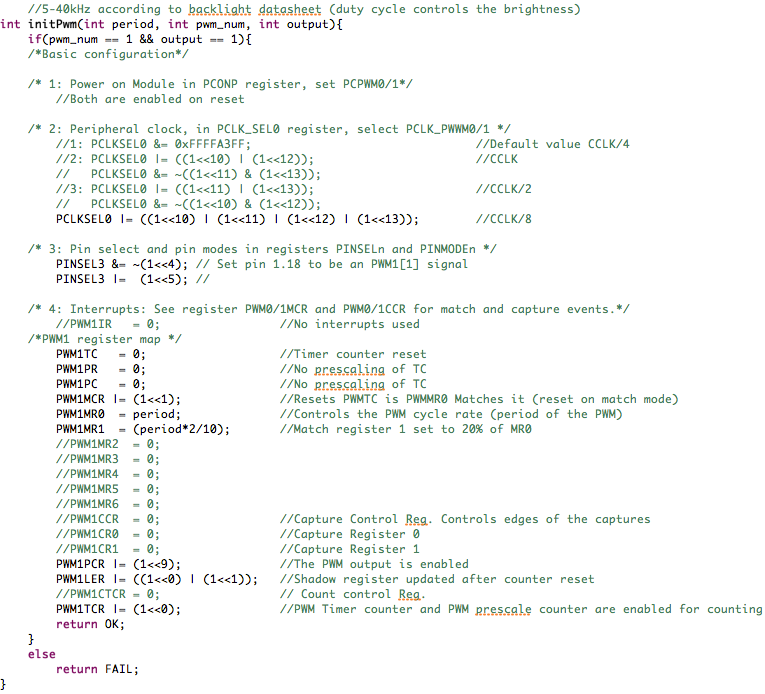
\includegraphics[width=0.93\textwidth]{init_pwm}
		\caption{All registers concerning the setup of a PWM signal is included in the initPwm function. The registers not used are
		commented out.}
	\end{centering}
\end{figure}
\newpage
The PWM signal on pin 1.18 is setup to reset on match. The MR0 register defines the pre scaling of the signal (as described in clock control).
The MR1 register is used to control the duty cycle of the PWM signal. To setup 50\% duty cycle, the MR1 register should be half the size of
MR0. For 100\% duty cycle the two registers should be equal and for 0\% duty cycle, the MR0 value should be 0.

\begin{figure}[h!]		%Remember to put the h!, to not fuck the sections.
	\begin{centering}
 		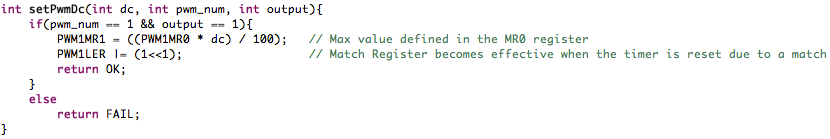
\includegraphics[width=1.0\textwidth]{set_pwm}
		\caption{Changing the duty cycle of a certain PWM signal.}
	\end{centering}
\end{figure}
As MR0 contains the maximum duty-cycle, it is included to calculate the step size when changing the duty-cycle.
After changing something in one of the MR registers, a pin in the LER (shadow register) should be set, to make the MR register update take effect. The value is changed after a reset (the "PWM counter" reaches its value).

\end{document}
